% -*- root: ../main.tex -*-
%modalità di divisione in itinere dei task, meeting/interazioni pianificate, modalità di revisione in itinere dei task, scelta degli strumenti di test/build/continuous integration
\chapter{Processo di Sviluppo}

\section{Domain Driven Design}
In questo capitolo viene analizzato il processo di sviluppo definito dal team. Fin dall'inizio, è stato scelto un approccio di design fortemente basato sul dominio. Infatti nella discussione preliminare sull'idea, sono emersi parecchi dubbi sul significato dei vocaboli usati e su concetti generali di funzionamento. Questo ha spinto il team ad avvalersi naturalmente di schemi per chiarificare e uniformare le astrazioni di ogni team-member. Questi schemi sono stati mantenuti e aggiornati per tutta la durata del progetto, uniformando l'artefatto generato con il modello del dominio. Questo permette anche la successiva evoluzione del progetto in modo più semplice.
    \subsection{Aspetti principali}
    I concetti chiave che hanno assunto particolare importanza nello sviluppo sono stati:
    \begin{itemize}
        \item \textbf{Domain Expert interview}: Per formalizzare le richieste e non permettere al software di allontanarsi da esse nello sviluppo l'intervista con l'esperto del dominio è stata formalizzata e trascritta assieme a tutte le domande (\ref{chap: IntervistaCommittente}).
        \item \textbf{Linguaggio Condiviso}: Per evitare continue spiegazioni tra i membri del team, per indicare a quale concetto si stesse facendo riferimento, è stata creata una tabella di "Ubiquitous Language" (\ref{chap:UbiquitousLanguage}).
        \item \textbf{User Stories}: Per assicurare che l'esperienza sia in linea con quella desiderata e che il software copra ogni interazione utente richiesta, sono state definite tutte le user stories che sono emerse dall'intervista con il committente (\ref{chap:UserStories}).
        \item \textbf{Mockup}: Per verificare che il team abbia carpito effettivamente l'aspettativa di risultato richiesta e il funzionamento sono stati sviluppati dei mockup, che il cliente ha verificato e approvato (\ref{chap:Mockup}).
    \end{itemize}


\section{Metodologia di Sviluppo}
Per sviluppare il progetto è stata scelto il framework Scrum. Infatti il processo di sviluppo è stato basato, in comune accordo, sulla metodologia agile. La motivazione risiede nel fatto che il team è composto da 4 persone e il prodotto deve essere sviluppato in tempi brevi. Il framework \textbf{Scrum} infatti permette di suddividere i compiti in maniera precisa, sviluppando il progetto in passi incrementali, senza incorrere in fraintendimenti o problemi di integrazione all'ultimo. La qualità dell'artefatto generato è quindi molto alta e i rischi di insoddisfazione del cliente sono minimi, grazie allo sviluppo ciclico che spezza il lavoro in piccoli goal e review. 
    \subsection{Scrum}. 
    Secondo il framework "Scrum" il lavoro deve essere diviso in più sprint seguendo un approccio iterativo. Per questo motivo l'intervallo di tempo disponibile per lo sviluppo del progetto è stato suddiviso in sotto-intervalli di una settimana. 
    Il team mantiene due tipi di backlog questi riflettono l'organizzazione temporale spiegata sopra: il product backlog e lo sprint backlog. 
    
    \paragraph{Product Backlog}Il product backlog racchiude il progresso generale del progetto, in cui ogni item riflette una user-story, o una funzionalità ad alto livello, di cui il cliente può apprezzare lo sviluppo. Queste vengono ordinate per urgenza e dimensione, e scelto un sottoinsieme, assegnate allo sprint successivo. In ogni sprint è presente infatti lo sprint backlog, in cui si può apprezzare in maniera molto più dettagliata e a basso livello l'implementazione delle varie feature. 

    \paragraph{Sprint Backlog} Lo sprint backlog, proprio di ogni intervallo, va a raffinare nella riunione iniziale (sprint planning) gli item scelti (sprint goal) dal product backlog. Questi sono suddivisi in più task e assegnati a diversi membri del team. Nel meeting finale (sprint review) lo sprint backlog viene ispezionato, riordinato e utilizzato per ulteriori considerazioni sull'iterazione successiva. Per maggiori dettagli sul processo di sviluppo per ogni iterazione si veda il capitolo \ref{chap:Retrospettiva}.

    \paragraph{Definition of done} Un item del product backlog o sprint backlog si ritiene concluso quando tutti i task che lo compongono sono stati completati, il codice implementato è stato adeguatamente testato con esito positivo e la relativa documentazione è stata scritta.
    
    \paragraph{Scrum poker} Per stimare il livello di effort necessario per il completamento di ogni task è stata utilizzata la tecnica che viene chiamata \textbf{scrum poker}. Questa tecnica consiste nella lettura e discussione di un task e degli aspetti che lo riguardano e nella scelta, da parte di ogni membro del team, di un valore di effort stimato scegliendo tra 1, 2, 3, 5, 8, 13, 20 il numero che ritiene più adeguato a rappresentare la complessità del task tenendo conto ad esempio del tempo ritenuto necessario per lo sviluppo o la complessità stimata del task stesso. A seguito della scelta di un numero da parte di ogni membro vengono rivelati i numeri scelti e si cerca di raggiungere consenso sulla scelta del numero finale, eventualmente argomentando la propria decisione. La scelta del set di numeri da assegnare è tale da avere volutamente ampi intervalli tra i numeri per ridurre conflitti e raggiungere con maggiore semplicità una situazione di consenso.

    \paragraph{Ruoli}
    I ruoli definiti da Scrum sono stati leggermente modificati, essendo il team composto da solo 4 persone. Nello specifico, il "domain-expert" e lo "scrum master" sono stati anche programmatori. 
    


\section{Gestione di Progetto}
In questa sezione verrà spiegato come il progetto è stato gestito con diversi tool seguendo la metodologia Scrum.
    \paragraph{Gantt Chart} 
    Per l'organizzazione del progetto con il Gantt è stato scelto \href{https://riccardo-omiccioli.atlassian.net/jira/software/projects/IQ/boards/1/roadmap}{Jira}. Questo tool ci ha permesso di avere una visione generale dei momenti del progetto, e quali task svolgere in ogni fase. Lo strumento inoltre è stato utile per la pianificazione e per mantenere la costanza attraverso le deadline. 
    
    \paragraph{Collaborative Design Board}
    Per le Board di Design è stato utilizzato \href{https://miro.com/app/board/uXjVPN93uLs=/?share_link_id=56431555728}{Miro} Lo strumento ci ha permesso di lavorare simultaneamente su grafici e schemi che sono stati molto utili nella fase iniziale di chiarificazione e design. 

    \paragraph{Product-Backlog}
    Per le Board di Scrum è stato utilizzato \href{https://github.com/orgs/ISIQuiz/projects/3}{GitHub-Projects} Il tool si è rivelato molto potente, grazie anche all'integrazione diretta con GitHub. La chiusura di issue avviene in maniera automatica al merge del branch relativo e gli item si spostano automaticamente nella board. Inoltre, la possibilità di avere diverse view su tutti i dati ha permesso di sviluppare product e sprint backlog senza ripetizioni o duplicazioni. Sono state create diverse view anche per facilitare i membri del team nell'osservare il progresso, la priorità e la grandezza dei task. I vari raffinamenti sono stati referenziati alle issue principali tramite la loro descrizione, in modo da poter osservare il completamento passo passo delle user-stories. Unica mancanza, è stato quello di poter assegnare delle issue a più sprint backlog, qualora non venissero completate in uno solo. 
    
    \paragraph{Licensing} 
    Per la licenza è stata scelta \href{https://choosealicense.com/licenses/}{la licenza base}
    
    \paragraph{Versioning}
    Riguardo al versioning, la piattaforme scelta è stata ovviamente Git. E per la sintassi, siccome il progetto è stato svolto in tempi ristetti, è stato scelto il versioning semantico unito a quello temporale, in cui ogni versione è rappresentata da MAJOR.MINOR.PATCH e dalla data in cui è stata implementata. Siamo consapevoli delle controindicazioni a riguardo del versioning temporale, del fatto che le date non rappresentino necessariamente il cambiamento del software e che non diano alcun grado di semantica su di esso, ma l'abbiamo trovata un'informazione utile soprattutto prima della consegna della prima Major, essendo il processo stabile e incrementale.
    
    \paragraph{Telegram}
    scelta Telegram...
        \subparagraph{Bot} 
        Telegram bot...
    
    \paragraph{Discord}
    Discord... 

\section{Continuous Integration e Automatizzazione}
\label{chap:CI}
Nel progetto la Continuous Integration (CI) e L'Automatizzazione delle mansioni più ripetitive hanno avuto notevole importanza. Una cospicua quantità di tempo è stata dedicata all'inizio per la messa in opera di pipeline che permettano di risparmiare tempo successivamente agli sviluppatori e di garantire la massima qualità al cliente finale.
    \subsection{Relazione}
        \subparagraph{Tool utilizzati}
        \begin{itemize}
            \item \LaTeX
            \item Overleaf
            \item GitHub Actions
            \item Telegram Bots
            \item Pandoc
            \item GitHub Pages
        \end{itemize}
        La relazione di progetto è stata svolta in \textbf{\LaTeX}. Questa decisione è motivata dal fatto che esso permette facilmente di organizzare lunghi testi in capitoli e sottocapitoli, eventualmente riordinando intere parti senza preoccuparsi dell'indice o della formattazione. Inoltre, permette la gestione in maniera più accurata, rispetto al Markdown, di elementi grafici, tabelle, stili, link e referenze, producendo un pdf finale molto più professionale. 
        
        Come strumento complementare è stato scelto \textbf{Overleaf}. La piattaforma permette di collaborare ininterrottamente e simultaneamente sullo stesso blocco di testo. Questo è risultato particolarmente utile nelle discussioni e nel produrre la documentazione negli "Sprint-planning" e, sopratutto, negli "Sprint-review". Particolarmente significative sono state le funzioni di poter generare immediatamente il pdf per osservare il risultato e poter raggiungere il cursore di altri membri del gruppo per osservare la documentazione prodotta in itinere. Ciò ha snellito molto il processo e ha eliminato laboriose review dei commit fatti con relativi commenti.  

        Dal lato "Continuous Integration", sono state sfruttate a pieno le \textbf{GitHub-Actions} messe a disposizione da GitHub. Queste permettono di generare il pdf finale in automatico e di renderlo pubblico con Release istantanee ad ogni cambiamento. Ciò ha non solo alleviato la preoccupazione di farlo manualmente, ma ha anche permesso di rendere disponibile al cliente sempre l'ultima versione aggiornata. 

        Per garantire la massima qualità, un \textbf{Bot Telegram} è stato utilizzato come strumento di notifica nel gruppo Telegram dedicato. Il Bot notifica come in [Fig. \ref{fig:ci-github}] qualora ci sia qualunque problema in ogni step della CI, altrimenti avverte che l'azione è stata portata a termine correttamente, inoltrando anche il pdf sul gruppo. 

        \begin{figure}[H]
            \caption{Pipeline GitHub Actions}
            \label{fig:ci-github}
            \centering
            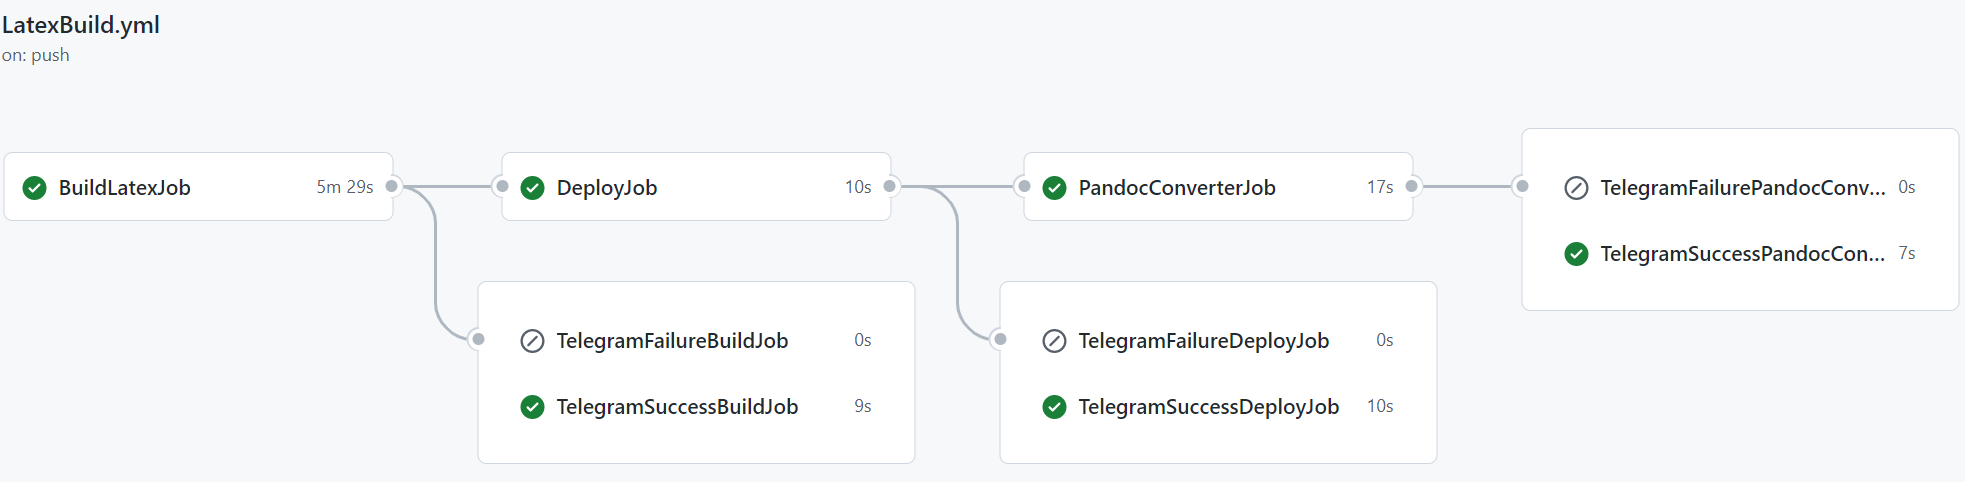
\includegraphics[width=1\textwidth]{Images/gh-pipeline.png}
        \end{figure}

        Qualora una persona volesse consultare la relazione online, senza scaricare il pdf, si è fatto uso di \textbf{Pandoc} per generare il relativo sito web, consultabile comodamente sul browser. Per la paginazione, un template html/css è stato utilizzato per rendere la vista più accattivante.

        Il deploy del sito, infine, è stato utilizzato \textbf{GitHub-Pages} che permette di semplificarne la messa in opera avendo un branch dedicato sul quale tutti i file relativi possono essere mantenuti e aggiornati.
        

    \subsection{Progetto}
        \subparagraph{Tool utilizzati}
        \begin{itemize}
            \item Sbt 1.7.2
            \item ScalaTest 3.2.14
            \item Sbt-assembly 2.0.0
            \item GitHub Actions
            \item GitHub Pages
            \item Telegram Bots
            \item Dependabot
            \item Sonarcloud/Codacy/Codefactor
            \item \href{https://riccardo-omiccioli.atlassian.net/jira/software/projects/IQ/boards/1/roadmap}{Jira}
            \item \href{https://miro.com/app/board/uXjVPN93uLs=/?share_link_id=56431555728}{Miro}
            \item \href{https://github.com/orgs/ISIQuiz/projects/3}{GitHub Boards}
            \item PlanItPoker \cite{planitpoker}
        \end{itemize}
    CI progetto, Test, Coverage, Documentazione, Quality assurance, bla bla

        \subsubsection{Quality Assurance}
        Per quanto riguarda la gestione di progetto con i vari branches, è stato scelto un branch develop su cui fare merge di ogni feature. Queste vengono implementate su branch a parte a partire dalle issue relative individuate nel refinement del Product Backlog. 
        Per garantire il giusto processo di sviluppo sono state attivate delle \textbf{Branch Protection Rules} che forzano la persona che contribuisce al codice a chiedere una pull request, prima di fare la merge forzosa da linea di comando. La pull request deve passare almeno una review da parte di altri sviluppatori, prima di essere introdotta nel branch di development. Inoltre sono stati introdotti gli status check, che vanno passati prima di poter fare la merge, questi comprendono il passare i test. 
        
    Per quanto riguarda la continuous integration del programma, come prima cosa è stato fatto il setup dello Scala Build Tool, specificando la versione di scala da utilizzare nel progetto, la versione di sbt stesso, inserendo le dipendenze di scalatest e il plugin sbt-assembly negli appositi file di configurazione. In modo analogo alla relazione, sono state poi utilizzate le GitHub actions per automatizzare la verifica dei test e per la release dei jar eseguibili. In particolare nell'immagine seguente è possibile osservare la pipeline eseguita ogni volta che delle nuove modifiche vengono spostate dal branch di develop al main branch.

    \begin{figure}[H]
        \caption{Pipeline progetto Scala}
        \label{fig:scala-ci-github}
        \centering
        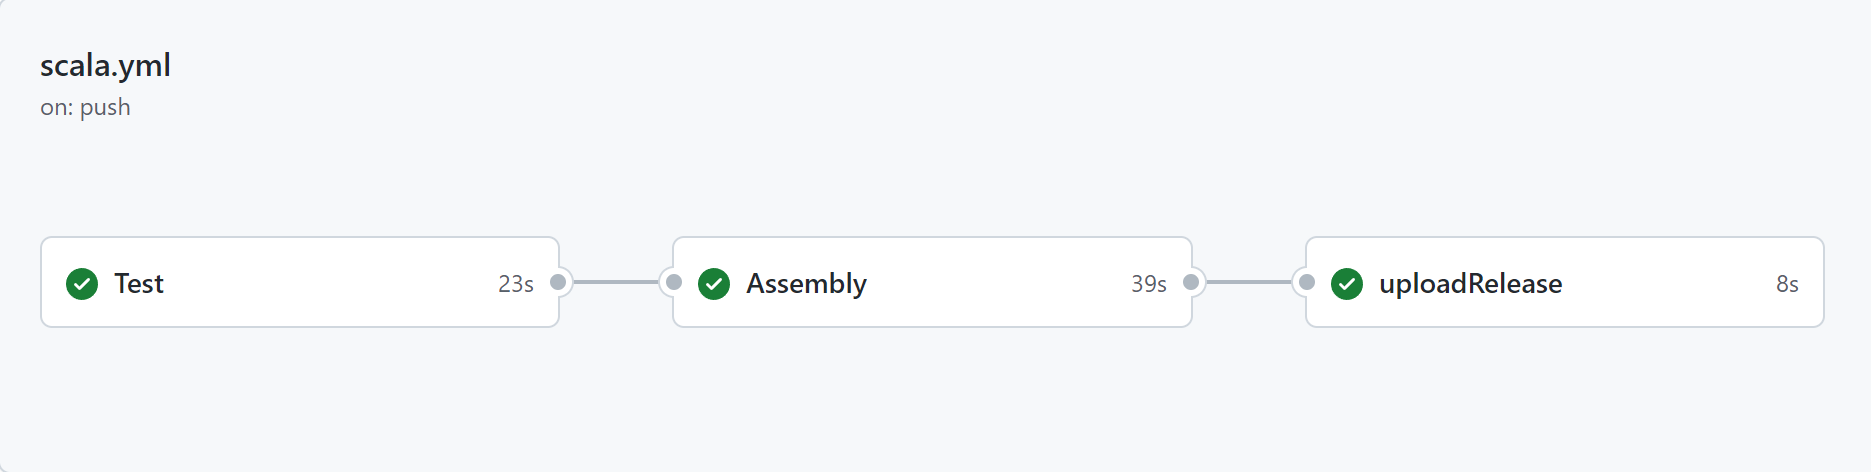
\includegraphics[width=1\textwidth]{Images/scalaCI-pipeline.png}
    \end{figure}

    La pipeline realizzata è strutturata in modo tale da eseguire tutti i test implementati e poi, solo in caso di successo della totalità di essi, la creazione dello uber jar (ovvero un jar contentene tutte le dipendenze e le risorse necessarie per l'esecuzione indipendente) sfruttando il plugin sbt-assembly. Il jar eseguibile realizzato viene infine caricato tra le release del progetto.






